\subsection{Dados de Lurian}
% p1q2 - 201601
% 

\begin{questions}
\question{
Lurian vai participar de um jogo de dados. Neste jogo, todos os dados
devem possuir 6 lados. Lurian é muito `esperta' e adiciona um pequeno peso a seu dado,
de forma que o lado 6 passe a ter probabilidade maior do que os demais.
Após utilizar este artifício, a função massa de probabilidade que rege o laçamento de seu dado
será $p = (p_1, \ldots, p_5, p_6) = \left( \frac{1}{7}, \ldots, \frac{1}{7}, \frac{2}{7} \right)$.
Desta forma, o lado de valor 6 terá o dobro da probabilidade que cada um dos demais.

\begin{parts}
\part
Calcule a entropia associada a um lance do dado de Lurian.

\part
Suponha que você queira gerar uma sequência de $m$ lances de dados, mas seria necessário que
o dado fosse honesto. Entretanto você dispõe apenas do dado fornecido por Lurian.
Proponha uma maneira de utilizar o dado fornecido por Lurian e gerar uma sequência
equivalente a uma sequencia proveniente de um dado honesto. Como podemos determinar
a abordagem para resolver este problema que forneça o menor \emph{overhead} 
\footnote{\emph{overhead}: custo excedente por unidade.}
possível?
% http://crypto.stackexchange.com/questions/29629/generating-unbiased-numbers-with-a-biased-six-sided-die
\end{parts}
}

\begin{solution}
\begin{parts}
\part
  \begin{eqnarray}
  H(X) &=& - \sum_{x \in \mathcal{X}} p(x) \log p(x) \nonumber \\
        &=& - 1/7 \times \log(1/7) - \ldots - 1/7 \times \log(1/7) - 2/7 \times \log(2/7) \nonumber \\
        &=& (5/7) \times \log(7) + (2/7) \times \log(7) - (2/7) \nonumber \\
        &=& \log(7) - (2/7) \approx 2.521
  \end{eqnarray}

\part 
Vamos mapear sequências de comprimento $n$ fornecidas pelo dado de Lurian em
sequências de comprimento $m$. De forma geral, devemos ter $n > m$, uma vez que
a entropia associada ao dado de Lurian é menor que a entropia de um dado honesto.
O \emph{overhead} será mínimo quando $n = m+1$ e tomando $m$ maior possível, de forma
a minimizar o \emph{overhead} que será de $1/m$. Devemos então encontrar o maior $m$ tal que $n=m+1$
e a entropia associada a uma sequência de comprimento $m$ para um dado honesto ($m H_1$, onde
$H_1$ é a entropia de um dado honesto e estamos considerando que os lances de dados são independentes)
deverá ser menor ou igual à entropia associada a uma sequência de comprimento $n$
para o dado de Lurian ($n H_2$, onde estamos chamando de $H_2$ a entropia associada ao lance do
dado de Lurian e considerando que os lances independentes).

\begin{lstlisting}[language=Octave]
% Lurian
p = [1/7 1/7 1/7 1/7 1/7 2/7];
H2 = - sum( p.* log2(p) )

% Honesto
p = 1/6 * ones(1,6);
H1 = - sum( p.* log2(p) )

m=[1:50]; r = m*H1./((m+1)*H2);
h = figure;
plot(m,r);
line([0 50], [1 1], 'LineStyle','--');
xlabel('m'); ylabel('r');
set(gca, 'Box', 'off');
print -dsvg dicelurian.svg;
system('inkscape dicelurian.svg --export-pdf=dicelurian.pdf');
\end{lstlisting}

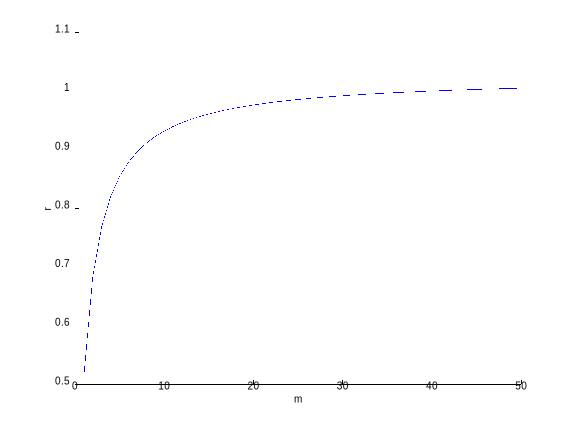
\includegraphics[width=0.5\textwidth]{../images/dicelurian.pdf}

Podemos verificar então que o valor máximo de $m$ é 39, para o qual
a relação $mH_1 \leq nH_2$ é satisfeita. Para este caso ($m=39$)
teremos um \emph{overhead} de apenas 2.5\%.

\end{parts}
\end{solution}
\end{questions}
